\chapter{Antecedentes}

\section{Modelo Estandar}

El Modelo Est\'andar es el formalismo te\'orico-experimental que hasta el d\'{\i}a de hoy  describe con mayor precisi\'on las interacciones entre las part\'{\i}culas elementales y los diferentes tipos de fuerzas que experimentan entre ellas. Los mayores desarrollos teorios y descrubrimientos que dieron forma al Modelo Estandar se dan a partir de la segunda mitad del siglo XX con el desarrollo de la Teoria Cuantica de Campo, fruto del esfuerzo de cientificos de todo el mundo, los cuales a partir de los modelos teoricos y observaciones experimentales construyeron una clasificaci\'on de las particulas en base a sus propiedades fundamentales como lo son la masa, la carga electrica, el espin, entre otras. Dicha clasificacion se muestra en la Figura~\ref{fig:ME}. Las part\'{\i}culas elementales son divididas en dos categor\'{\i}as, los fermiones y los bosones, los fermiones est\'an a su vez divididos en quarks y leptones los cuales tienen un valor fraccional de espin (1/2), adem\'as de que obedecen la estadistica de Fermi-Dirac y el principio de exclusion de Pauli. Los quarks son particulas elementales que constituyen a los hadrones, ya que debido al principio de confinamiento los quarks no pueden co-existir en estado libre.

Cuatro son las fuerzas fundamentales en la naturaleza, la fuerza electromagnetica, la debil, la fuerte y la gravitacional, el modelo estandar incluye las tres primeras, la gravitacional no esta incluida sin embargo su contribucion en la fisica de particulas es despreciable si se compara por ejemplo con la fuerza electromagnetica (una razon de $10^{36}$ a la escala de Giga-electron volts). El modelo estandar esta respaldado por una serie de observacines experimentales, la mas reciente la observaci\'on del boson de Higgs en 2012. Sin embargo aun existen fen\'omenos en la naturaleza que no pueden ser explicados con este formalismo, ejemplo de ellos son: La composicion y naturaleza de la materia y energia oscura.

\begin{figure}
\begin{center}
  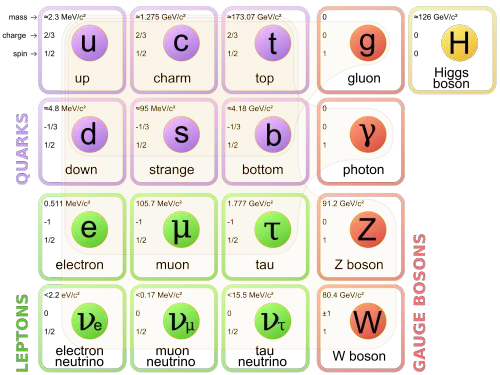
\includegraphics[width=4.0in]{standard-model.png}
  \caption{Clasificaci\'on de las particulas segun El Modelo est\'andar de las part\'iculas elementales}
  \label{fig:ME}
\end{center}
\end{figure}


\section{Materia Oscura}

La materia oscura o dark matter (por su nombre en ingles) recibe este nombre debido a que no se observa que emita radiaci\'on electromagn\'etica, por lo que su existencia se infiere debido a la influencia gravitacional sobre la materia visible o tambien conocida como barionica que se encuentra a su alrededor, dicho fenomeno ha sido observado en cumulos de galaxias en donde la velocidad de rotacion de las mismas no corresponde a la que seria producida debido a la fuerza de gravedad ejercida por la materia visible a su alrededor. A pesar de los esfuerzos por parte de la comunidad cientifica hasta este momento se desconoce la composicion de la materia oscura, lo que se sabe, por medio de observacones astronomicas, es que aproximadamente la materia oscura representa el 30.1\%  de la composici\'on materia-energia del universo, el resto es energia oscura (69.4\%) y materia visible (0.5\%). Recientemente y con el afan de entender la composicion de la materia oscura y su localizacion en el universo la comunidad cientifica ha desarrollado varios experientos, uno de los mas significativos es el Alpha Magnetic Spectrometer (AMS-02) el cual es un detector, el cual entre sus objetivos mas importantes es el de buscar indicios de materia oscura y antimateria, dicho detector fue disenado en el laboratorio CERN y fue instalado en la estacion espacial internaciona (ISS por sus siglas en ingles). En sus observaciones mas recientes se ha observado un flujo de positrones anomalo el cual podria ser explicado como el producto de aniquilacion de particulas de materia oscura~\cite{ams:cern}.  Dicho flujo anomalo puede observarse en la Figura~\ref{fig:AMS_positron} donde tambien se presenta una comparacion con otros experimentos que observan similar comportamiento.  El exceso de flujo puede ser observado a partir de los 25 GeV. 


\begin{figure}
\begin{center}
 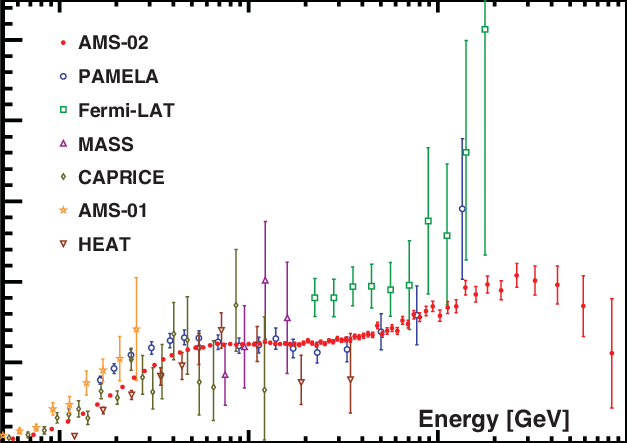
\includegraphics[width=4.0in]{AMS_positronflux.png}
  \caption{Flujo de positrones medido por el experimento AMS-02, comparado con los experimentos PAMELA,Fermi-LAT, MASS, CAPIRCE, AMS-01 y HEAT.}
 \label{fig:AMS_positron}
 \end{center}
\end{figure}

Dichas observaciones cosmologicas han motivado a los fisicos teoricos 
altas energias a postular nuevos modelos en los cuales la composicion de la materia oscura se pueda enterder por medio de nuevas particulas elementales  las cuales podrian estar siendo actualmente producidas en los aceleradores de particulas modernos como lo es el Gran Colisionador de Hadrones en Ginebra, Suiza.  Dichos modelos entran en la categoria de extensiones al modelo estandar y por lo general involucran la existencia de nuevas particulas cuyas fuerzas e interacciones estan descritas por alguna variacion de la Teoria Cuantica de Campo, lo que sugiere que su produccion y propiedades pueden ser estudiadas por el formalismo de la fisica de particulas y la parte experimental por medio de los detectores de particulas lo cual involucra tecnicas de recoleccion de datos, seleccion de eventos y tecnicas estadisticas para extraccion de posibles senales.  

\chapter{Propuesta}

En este trabajo se propone hacer un estudio de varios modelos teoricos, clasificados como extensiones al modelo estandar, y que predicen la creacion de nuevas particulas como producto de las colisiones de protones altamente energeticos. Estas nuevas particulas serian candidatos a explicar la composicion de la materia oscura.  Usualmente en dichos modelos las nuevas particulas interacciones debilmente con la materia barionica por lo que su deteccion se daria de forma indirecta, es decir, por su decaimiento a particulas conocidas del modelo estandar.  Adicionalmente al estudio de los modelos teoricos se pretende trabajar en la parte experimental, la cual consiste en el estudio de la respuesta del detector al paso de las particulas elementales.  La parte experimental es fundamental ya que sin una buena estrategia de seleccion de datos, tecnicas de supresion de ruido y optimizacion de senal seria imposible la observacion de nueva fisica. En este proyecto se considera el detector CMS del CERN como el aparato experimental que proporcionara los datos de estudio, ya sea por simulacion o por uso de datos reales.  

El Experimento CMS es uno de los detectores multi usos del CERN el cual cubre un amplio rango de procesos fisicos que se pueden estudiar, dicho experimento, junto con el experimento ATLAS pudieron observar la particula de Higgs en el 2012.  El experimento consiste de subsistemas los cuales estan disenados para la identifcacion de todas las particulas del modelo estandar, disenado desde suc onstruccion deacuerdo a como cada particula interacciona con la materia, por ejemplo las particulas cargadas son detectadas por detectores de silicio y detectores de gas, ademas de que el signo de la carga es determinado deacuerdo a la defleccion en el campo magnetico solenoide de 4 Teslas.  Las particulas neutras son identificadas por la energia que depositan en los calorimetos.   

En este estuddio se propone el estudio de las senales de nuevas particulas y su paso por el detector por medio de simulacion, de esta manera optimizar la seleccion de los eventos en base a las propiedades de cada modelo, en una segunda fase se pretende estudiar la senal de dichos modelos bajo diferentes escenarios del detector CMS, es decir con el actual detector usado hasta el 2018, durante el llamado periodo 'Run-2'' y el detector que esta disenado para la fase de alta luminosidad, o tambien llamada Phase-2, la cual empezara  a partir del 2025, de esta manera se puede predecir en base a los estudios de simulacion las posibilidades de identificacion de una nueva senal en los proximos anios. 

Dicho estudio es bastante propicio debido a la relevancia de la etapa de alta luminosidad en donde la frecuencia de datos que se acumulara aumentara un factor de 10, es decir la probabilidad de deteccion de nuevas senales sera mucho mayor que la que se tienen con los datos recolectados actualemente, especialmente para el tipo de senales que se desea estudiar. 


\chapter{Justificacion}

Actualmente los modelos teoricos que predicen la formacion de particulas de materia oscura no han sido explorada ampliamente, en gran medida por falta de datos exprimentales que permitan explorar el espacio fase que dichos modelos predicen para esas particulas.  Actualmente con el funcionamiento del gran acelerador de hadrones y sus proyecciones en cuanto a recoleccion de datos en lo proximos anios es la perffecta oportunidad para explotar lo ms posible el estudio de dichos modelos, para en dado caso descubir una nueva senal o en su defecto exlcluir el espacio fase de las particulas predichas. 

\chapter{Hipotesis}

La hipotesis que se maneja en este estudio se basa en que la materia oscura esta compuesta de particulas elementales las cuales pueden ser producidas en el laboratorio, de ser esto posible se requiere de una extension al modelo estandar, es decir un modelo teorico que de sustento a dicha hipotesis. Afortunadamente ya existenn varias modelos teoricos que predicen dicho fenomeno, uno de los mas populares el el llamado sector oscuro, o dark sector por sus siglas en ingles, en el cual debido al rompimiento de una simetria se da lugar a la produccion del llamado foton oscuro (dark photon), dicha particula seria la portadora entre el sector oscuro y el del modelo estandar y la interaccion entre estos dos sectores se daria por medio de lo que se conoce como el parametro kinetico de mezcla (kinetic mixing paramette), usualmente abreviado como $\epsilon$. 

Una de las caracteristicas de esta nueva particula y que la diferencia del foton del modelo estandar es que seria masiva y que su tiempoo de vida podria ser significativo, ademas de que su interaccion se daria de forma indirecta, es decir por el decaimiento a particulas del modelo estandar.  Uno de los canales mas prometedores es en el que el foton oscuro decae a muones. los muones son particulas que pueden ser identificadas y reconstruidas con gran eficacia usando el detector CMS por lo que la probabilidad de deteccion es mayor que on otros modos de decaimientos.

\begin{figure}
\begin{center}
  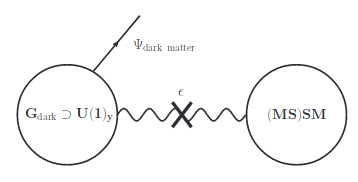
\includegraphics[width=2.8in]{sketch_darksector.png}
  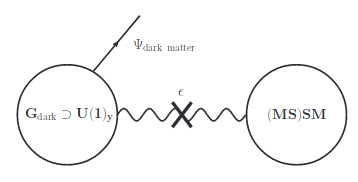
\includegraphics[width=2.8in]{sketch_darksector.png}
  \caption{Ilustracion esquematica de la conexion entre el sector oscuro y el modelo estandar, los cuales estan conectados mediente un termino de mezcla dinamica $\epsilon$}
  \label{fig:AMS_positron}
\end{center}
\end{figure}


\chapter{Objetivo General}

El objetivo principal de este proyecto es que se realice un estudio principalmente por medio de simulacion de montecarlo de diferentes modelos teoricos que postulan candidatos a particulas que den una explicacion de la naturaleza de la materia oscura.   Se busca lograr extraer la probabilidad de deteccion de dicha senal en los proximos anios usando como escenario las condiciones experimentales del experimento CSM del CERN.   Se pretende que dicho trabajo de simulacion sirva de base para un trabajo futuro mas detallado donde se incorporen tecnicas mas avanzadas de estudio. 


\chapter{Objetivos Especificos}

Los objetivos especificos del proyecto se enlistan a continuacion: 

\begin{itemize}
    \item Aprender a manipular los paquetes MadGraph y Pythia los cuales son usados por la comuidad de altas energias y sirven como herramienta fundamental para el estudio de nuevos modelos de fisica teorica.
    \item Utilizacion del paquete de simulacion Delphes el cual recrea el paso de las particulas por el detector, permite obtener eficiencias de identificacion y reconstruccion de particulas, aso como la intensidad de la senal con respecto al ruido
   \item Estudiar los diferentes escenarios experimentales, lo cual incluye el estudio de la deteccion de senales con el detector actual y con las futuras actualizaciones
\end{itemize}


\chapter{Metodología}

Para lograr cubrir los objetivos del proyecto el estudiante seguria una seria de pasos los cuales se encuentra resumidos a continuacion:

Produccion de muestras de MonteCarlo: Se espera producir muestras de simulacion de monte carlo para cada proceso de la se\~nal y ruido, el numero de eventos a producir depende del tipo de proceso que se este estudiando y su seccion eficaz, a menor seccion eficaz mayor numero de eventos que se necesitaran producir, las muestras se espera se produzcan usando los recursos computacionales de la Universidad de Sonora. Dicho paso requiere del desarrollo de codigo para la distribucion de las corridas de simulacion en forma paralela usando el cluster ACARUS. Los paquetes de simulacion que se usaran seran MADGRAPH~\cite{Alwall:2007st}, Pythia y Delphes~\cite{deFavereau2014}.

Analisis preliminar: El estudiante debe desarrollar diferentes herrammientas de analisis de datos, con el fin de acceder a los datos producidos en la simulacion y extraer las variables de interes, comunmente dichas herramientas de analisis consisten de codigos escritos en lenguaje C++ y python, de esta manera el estudiante dearrollara habilidad en la manipulacion de muestras de datos 

Seleccion de eventos: Despues del acceso de dataos de simulacion y variables de interes se procedera al estudio de la seleccion de eventos, la cual a grandes razgos consiste en seleccionar el conjunto de variables fisicas y valores los cuales puedan optimizar el proceso de senal y reducir lo mas posible la contribucion de ruido 

Analisis estadistico: Despues de la seleccion de eventos se realizara un estudio estadistico en el cual se extraeran el numero de eventos de senal y ruido despues de la seleccion, de ahi se puede interpretar los resultados en base a indicadores estadisticos y concluir la probabibilidad de obsservacion con datos recolectados en los siguientes anos terminao de


\chapter{Resultados Esperados} 

etar en De los estudios de simulaci\'on se espera obtener los siguientes resultados

\begin{itemize}
\item Caracterizacion de los diferentes parametros de los modelos estudiados, asi como las propiedades kinematicas de las diferentes particulas 
\item Las eficiencias de identificacion de particulas 
\item La eficiencia de reconstruccion de particulas 
\item La razon de la senal contra el ruido 
\item La sensitividad de descubrimiento para la etapa de alta luminosidad del experimento CMS
\end{itemize}




